% Created by tikzDevice version 0.8.1 on 2015-11-15 20:54:59
% !TEX encoding = UTF-8 Unicode
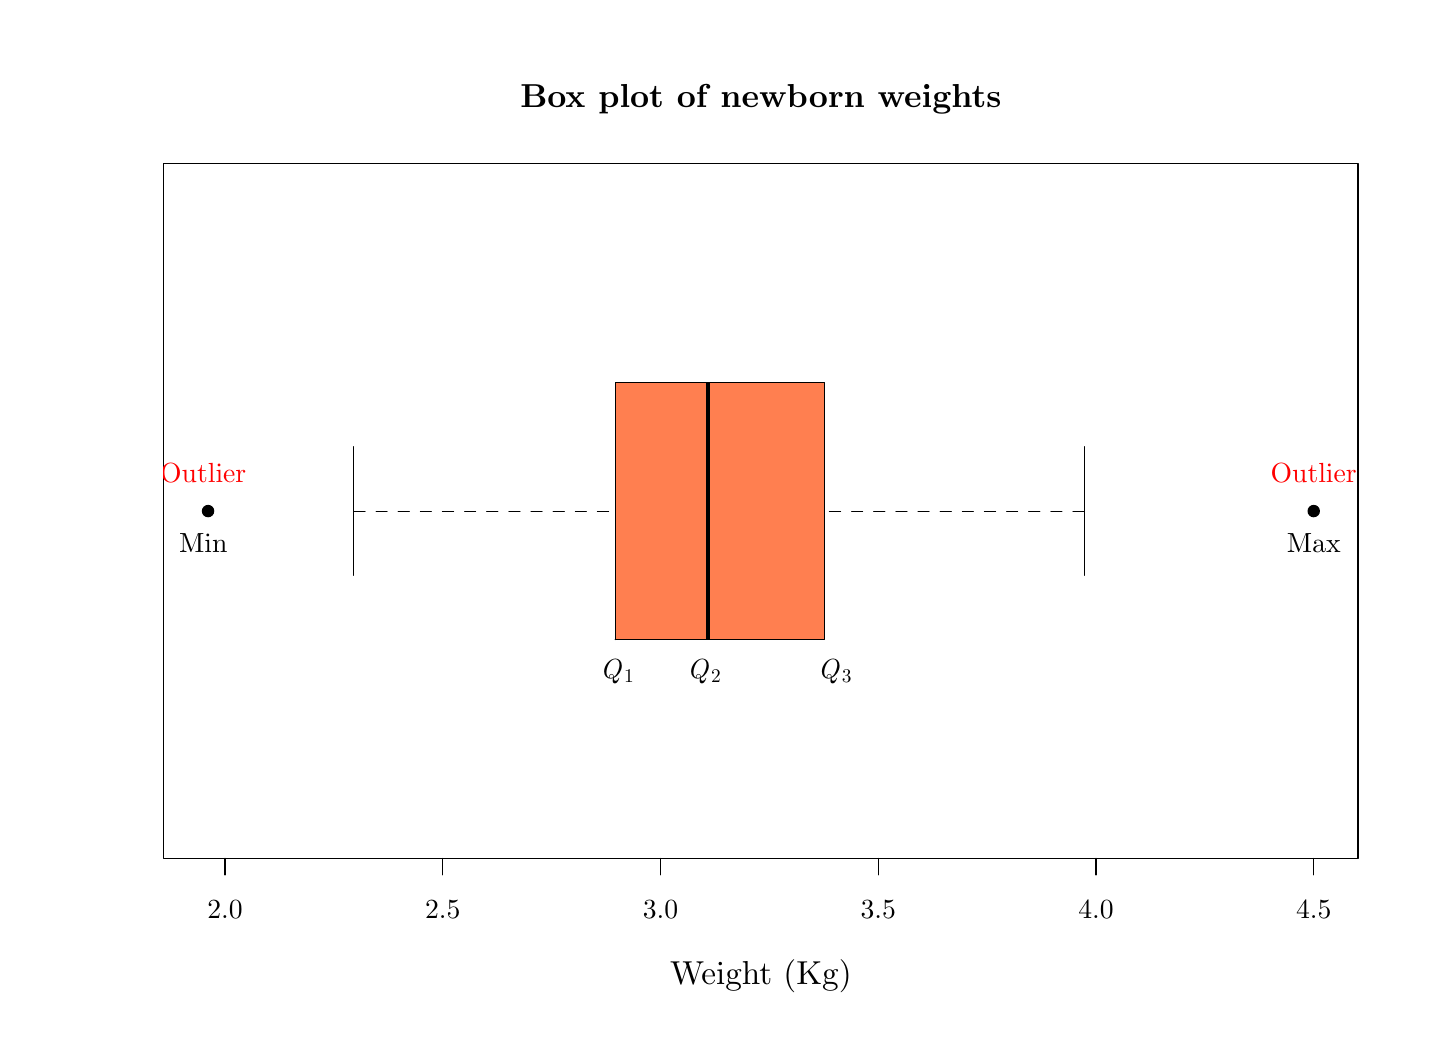
\begin{tikzpicture}[x=1pt,y=1pt]
\definecolor{fillColor}{RGB}{255,255,255}
\path[use as bounding box,fill=fillColor,fill opacity=0.00] (0,0) rectangle (505.89,361.35);
\begin{scope}
\path[clip] ( 49.20, 61.20) rectangle (480.69,312.15);
\definecolor{fillColor}{RGB}{255,127,80}

\path[fill=fillColor] (212.32,140.20) --
	(212.32,233.15) --
	(287.95,233.15) --
	(287.95,140.20) --
	cycle;
\definecolor{drawColor}{RGB}{0,0,0}

\path[draw=drawColor,line width= 1.2pt,line join=round] (245.85,140.20) -- (245.85,233.15);

\path[draw=drawColor,line width= 0.4pt,dash pattern=on 4pt off 4pt ,line join=round,line cap=round] (117.89,186.67) -- (212.32,186.67);

\path[draw=drawColor,line width= 0.4pt,dash pattern=on 4pt off 4pt ,line join=round,line cap=round] (381.73,186.67) -- (287.95,186.67);

\path[draw=drawColor,line width= 0.4pt,line join=round,line cap=round] (117.89,163.44) -- (117.89,209.91);

\path[draw=drawColor,line width= 0.4pt,line join=round,line cap=round] (381.73,163.44) -- (381.73,209.91);

\path[draw=drawColor,line width= 0.4pt,line join=round,line cap=round] (212.32,140.20) --
	(212.32,233.15) --
	(287.95,233.15) --
	(287.95,140.20) --
	(212.32,140.20);
\definecolor{fillColor}{RGB}{0,0,0}

\path[fill=fillColor] ( 65.18,186.67) circle (  2.25);

\path[fill=fillColor] (464.71,186.67) circle (  2.25);
\end{scope}
\begin{scope}
\path[clip] (  0.00,  0.00) rectangle (505.89,361.35);
\definecolor{drawColor}{RGB}{0,0,0}

\path[draw=drawColor,line width= 0.4pt,line join=round,line cap=round] ( 71.31, 61.20) -- (464.71, 61.20);

\path[draw=drawColor,line width= 0.4pt,line join=round,line cap=round] ( 71.31, 61.20) -- ( 71.31, 55.20);

\path[draw=drawColor,line width= 0.4pt,line join=round,line cap=round] (149.99, 61.20) -- (149.99, 55.20);

\path[draw=drawColor,line width= 0.4pt,line join=round,line cap=round] (228.67, 61.20) -- (228.67, 55.20);

\path[draw=drawColor,line width= 0.4pt,line join=round,line cap=round] (307.35, 61.20) -- (307.35, 55.20);

\path[draw=drawColor,line width= 0.4pt,line join=round,line cap=round] (386.03, 61.20) -- (386.03, 55.20);

\path[draw=drawColor,line width= 0.4pt,line join=round,line cap=round] (464.71, 61.20) -- (464.71, 55.20);

\node[text=drawColor,anchor=base,inner sep=0pt, outer sep=0pt, scale=  1.00] at ( 71.31, 39.60) {2.0};

\node[text=drawColor,anchor=base,inner sep=0pt, outer sep=0pt, scale=  1.00] at (149.99, 39.60) {2.5};

\node[text=drawColor,anchor=base,inner sep=0pt, outer sep=0pt, scale=  1.00] at (228.67, 39.60) {3.0};

\node[text=drawColor,anchor=base,inner sep=0pt, outer sep=0pt, scale=  1.00] at (307.35, 39.60) {3.5};

\node[text=drawColor,anchor=base,inner sep=0pt, outer sep=0pt, scale=  1.00] at (386.03, 39.60) {4.0};

\node[text=drawColor,anchor=base,inner sep=0pt, outer sep=0pt, scale=  1.00] at (464.71, 39.60) {4.5};
\end{scope}
\begin{scope}
\path[clip] (  0.00,  0.00) rectangle (505.89,361.35);
\definecolor{drawColor}{RGB}{0,0,0}

\node[text=drawColor,anchor=base,inner sep=0pt, outer sep=0pt, scale=  1.20] at (264.94,332.61) {\bfseries Box plot of newborn weights};

\node[text=drawColor,anchor=base,inner sep=0pt, outer sep=0pt, scale=  1.20] at (264.94, 15.60) {Weight (Kg)};
\end{scope}
\begin{scope}
\path[clip] (  0.00,  0.00) rectangle (505.89,361.35);
\definecolor{drawColor}{RGB}{0,0,0}

\path[draw=drawColor,line width= 0.4pt,line join=round,line cap=round] ( 49.20, 61.20) --
	(480.69, 61.20) --
	(480.69,312.15) --
	( 49.20,312.15) --
	( 49.20, 61.20);
\end{scope}
\begin{scope}
\path[clip] ( 49.20, 61.20) rectangle (480.69,312.15);
\definecolor{drawColor}{RGB}{0,0,0}

\node[text=drawColor,anchor=base west,inner sep=0pt, outer sep=0pt, scale=  1.00] at (206.83,126.11) {\itshape Q};

\node[text=drawColor,anchor=base west,inner sep=0pt, outer sep=0pt, scale=  0.70] at (215.53,124.61) {1};

\node[text=drawColor,anchor=base west,inner sep=0pt, outer sep=0pt, scale=  1.00] at (238.31,126.11) {\itshape Q};

\node[text=drawColor,anchor=base west,inner sep=0pt, outer sep=0pt, scale=  0.70] at (247.00,124.61) {2};

\node[text=drawColor,anchor=base west,inner sep=0pt, outer sep=0pt, scale=  1.00] at (285.51,126.11) {\itshape Q};

\node[text=drawColor,anchor=base west,inner sep=0pt, outer sep=0pt, scale=  0.70] at (294.21,124.61) {3};

\node[text=drawColor,anchor=base,inner sep=0pt, outer sep=0pt, scale=  1.00] at ( 63.44,171.61) {Min};

\node[text=drawColor,anchor=base,inner sep=0pt, outer sep=0pt, scale=  1.00] at (464.71,171.61) {Max};
\definecolor{drawColor}{RGB}{255,0,0}

\node[text=drawColor,anchor=base,inner sep=0pt, outer sep=0pt, scale=  1.00] at ( 63.44,197.17) {Outlier};

\node[text=drawColor,anchor=base,inner sep=0pt, outer sep=0pt, scale=  1.00] at (464.71,197.17) {Outlier};
\end{scope}
\end{tikzpicture}
